\documentclass[journal,12pt,twocolumn]{IEEEtran}

\usepackage{graphicx}
\graphicspath{ {./5600/} }
\usepackage{amsmath}
\newcommand{\myvec}[1]{\ensuremath{\begin{pmatrix}#1\end{pmatrix}}}
\title{ Assignment1}
\author{PARIMISETTY HARINADHA (CS19RESCH11004)}
\begin{document}
\maketitle
\newpage
\begin{abstract}
This document explains the concept of collinear and whether the triangle formed by given 3 points is right angled triangle or not.
\end{abstract}
Download all python codes from 
\framebox[1\width]{ https://github.com/cs19resch11004/5600/hari }
Download all Latex-tikz codes from 
\framebox[1.1\width]{ https://github.com/cs19resch11004/5600/hari} 
\section{Problem}
Without using the Pythagoras theorem, show that \myvec{ 4 \\ 4 }, \myvec{ 3 \\ 5 } and \myvec{ -1 \\ -1 } are the vertices of a right angled triangle?

\section{Solution}
The direction vectors of $\vec{A}-\vec{B}$, $\vec{A}-\vec{C}$ and $\vec{B}-\vec{C}$ are
\begin{align}
	\vec{A}-\vec{B} =\myvec{-1 \\ 1} \\
	\vec{A}-\vec{C} =\myvec{-5 \\ -5}\\
	\vec{B}-\vec{C} =\myvec{-4 \\ -6} 
\end{align}
\begin{enumerate}
\item \begin{align} {(\vec{A}-\vec{B})}^T  (\vec{B}-\vec{C})  =   \myvec{ -1 \\ 1 }  \myvec{ -4 \\ -6 } = -2 \end{align}
\begin{align}{(\vec{A}-\vec{B})}^T  (\vec{B}-\vec{C}) = -2 \neq 0 \end{align}
Sides $\vec{A}-\vec{B}$ and $\vec{B}-\vec{C}$ of triangle are not perpendicular.

\item \begin{align}{(\vec{A}-\vec{C})}^T  (\vec{B}-\vec{C}) =  \myvec{ -5 \\ -5 }  \myvec{ -4 \\ -6 } = 50\end{align}
\begin {align}{(\vec{A}-\vec{C})}^T  (\vec{B}-\vec{C}) = 50 \neq 0 \end {align}
Sides $\vec{A}-\vec{C}$ and $\vec{B}-\vec{C}$ of triangle are not perpendicular.

\item \begin{align}{(\vec{A}-\vec{B})}^T  (\vec{A}-\vec{C}) =  \myvec{ -1 \\ 1 }  \myvec{ -5 \\ -5 } = 0\end{align}
\begin {align}{(\vec{A}-\vec{B})}^T  (\vec{A}-\vec{C}) = 0  \end {align}
Sides $\vec{A}-\vec{B}$ and  $\vec{A}-\vec{C}$  of triangle are perpendicular to each other and the right angle at vertex \myvec{ 4 \\ 4 }, and the following figure represents the triangle formed by given points $\vec{A}$, $\vec{B}$ and $\vec{C}$.  
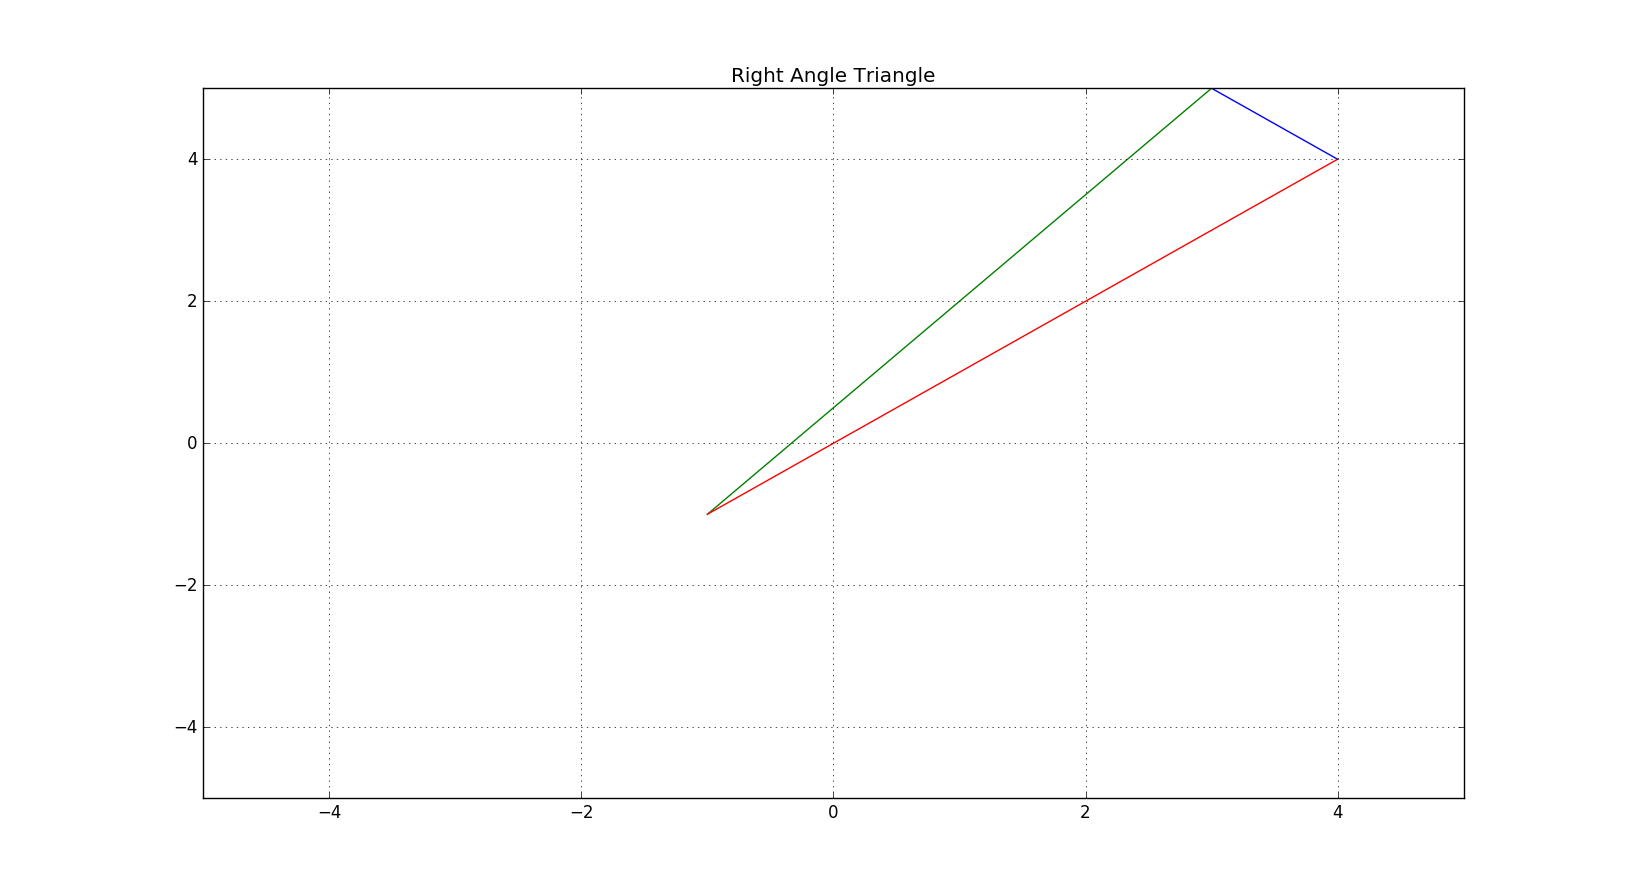
\includegraphics[width=11cm, height=7cm]{vihi}
\end{enumerate}
\end{document}
